% Options for packages loaded elsewhere
\PassOptionsToPackage{unicode}{hyperref}
\PassOptionsToPackage{hyphens}{url}
\PassOptionsToPackage{dvipsnames,svgnames,x11names}{xcolor}
%
\documentclass[
  letterpaper,
  DIV=11,
  numbers=noendperiod]{scrreprt}

\usepackage{amsmath,amssymb}
\usepackage{iftex}
\ifPDFTeX
  \usepackage[T1]{fontenc}
  \usepackage[utf8]{inputenc}
  \usepackage{textcomp} % provide euro and other symbols
\else % if luatex or xetex
  \usepackage{unicode-math}
  \defaultfontfeatures{Scale=MatchLowercase}
  \defaultfontfeatures[\rmfamily]{Ligatures=TeX,Scale=1}
\fi
\usepackage{lmodern}
\ifPDFTeX\else  
    % xetex/luatex font selection
\fi
% Use upquote if available, for straight quotes in verbatim environments
\IfFileExists{upquote.sty}{\usepackage{upquote}}{}
\IfFileExists{microtype.sty}{% use microtype if available
  \usepackage[]{microtype}
  \UseMicrotypeSet[protrusion]{basicmath} % disable protrusion for tt fonts
}{}
\makeatletter
\@ifundefined{KOMAClassName}{% if non-KOMA class
  \IfFileExists{parskip.sty}{%
    \usepackage{parskip}
  }{% else
    \setlength{\parindent}{0pt}
    \setlength{\parskip}{6pt plus 2pt minus 1pt}}
}{% if KOMA class
  \KOMAoptions{parskip=half}}
\makeatother
\usepackage{xcolor}
\setlength{\emergencystretch}{3em} % prevent overfull lines
\setcounter{secnumdepth}{5}
% Make \paragraph and \subparagraph free-standing
\ifx\paragraph\undefined\else
  \let\oldparagraph\paragraph
  \renewcommand{\paragraph}[1]{\oldparagraph{#1}\mbox{}}
\fi
\ifx\subparagraph\undefined\else
  \let\oldsubparagraph\subparagraph
  \renewcommand{\subparagraph}[1]{\oldsubparagraph{#1}\mbox{}}
\fi

\usepackage{color}
\usepackage{fancyvrb}
\newcommand{\VerbBar}{|}
\newcommand{\VERB}{\Verb[commandchars=\\\{\}]}
\DefineVerbatimEnvironment{Highlighting}{Verbatim}{commandchars=\\\{\}}
% Add ',fontsize=\small' for more characters per line
\usepackage{framed}
\definecolor{shadecolor}{RGB}{241,243,245}
\newenvironment{Shaded}{\begin{snugshade}}{\end{snugshade}}
\newcommand{\AlertTok}[1]{\textcolor[rgb]{0.68,0.00,0.00}{#1}}
\newcommand{\AnnotationTok}[1]{\textcolor[rgb]{0.37,0.37,0.37}{#1}}
\newcommand{\AttributeTok}[1]{\textcolor[rgb]{0.40,0.45,0.13}{#1}}
\newcommand{\BaseNTok}[1]{\textcolor[rgb]{0.68,0.00,0.00}{#1}}
\newcommand{\BuiltInTok}[1]{\textcolor[rgb]{0.00,0.23,0.31}{#1}}
\newcommand{\CharTok}[1]{\textcolor[rgb]{0.13,0.47,0.30}{#1}}
\newcommand{\CommentTok}[1]{\textcolor[rgb]{0.37,0.37,0.37}{#1}}
\newcommand{\CommentVarTok}[1]{\textcolor[rgb]{0.37,0.37,0.37}{\textit{#1}}}
\newcommand{\ConstantTok}[1]{\textcolor[rgb]{0.56,0.35,0.01}{#1}}
\newcommand{\ControlFlowTok}[1]{\textcolor[rgb]{0.00,0.23,0.31}{#1}}
\newcommand{\DataTypeTok}[1]{\textcolor[rgb]{0.68,0.00,0.00}{#1}}
\newcommand{\DecValTok}[1]{\textcolor[rgb]{0.68,0.00,0.00}{#1}}
\newcommand{\DocumentationTok}[1]{\textcolor[rgb]{0.37,0.37,0.37}{\textit{#1}}}
\newcommand{\ErrorTok}[1]{\textcolor[rgb]{0.68,0.00,0.00}{#1}}
\newcommand{\ExtensionTok}[1]{\textcolor[rgb]{0.00,0.23,0.31}{#1}}
\newcommand{\FloatTok}[1]{\textcolor[rgb]{0.68,0.00,0.00}{#1}}
\newcommand{\FunctionTok}[1]{\textcolor[rgb]{0.28,0.35,0.67}{#1}}
\newcommand{\ImportTok}[1]{\textcolor[rgb]{0.00,0.46,0.62}{#1}}
\newcommand{\InformationTok}[1]{\textcolor[rgb]{0.37,0.37,0.37}{#1}}
\newcommand{\KeywordTok}[1]{\textcolor[rgb]{0.00,0.23,0.31}{#1}}
\newcommand{\NormalTok}[1]{\textcolor[rgb]{0.00,0.23,0.31}{#1}}
\newcommand{\OperatorTok}[1]{\textcolor[rgb]{0.37,0.37,0.37}{#1}}
\newcommand{\OtherTok}[1]{\textcolor[rgb]{0.00,0.23,0.31}{#1}}
\newcommand{\PreprocessorTok}[1]{\textcolor[rgb]{0.68,0.00,0.00}{#1}}
\newcommand{\RegionMarkerTok}[1]{\textcolor[rgb]{0.00,0.23,0.31}{#1}}
\newcommand{\SpecialCharTok}[1]{\textcolor[rgb]{0.37,0.37,0.37}{#1}}
\newcommand{\SpecialStringTok}[1]{\textcolor[rgb]{0.13,0.47,0.30}{#1}}
\newcommand{\StringTok}[1]{\textcolor[rgb]{0.13,0.47,0.30}{#1}}
\newcommand{\VariableTok}[1]{\textcolor[rgb]{0.07,0.07,0.07}{#1}}
\newcommand{\VerbatimStringTok}[1]{\textcolor[rgb]{0.13,0.47,0.30}{#1}}
\newcommand{\WarningTok}[1]{\textcolor[rgb]{0.37,0.37,0.37}{\textit{#1}}}

\providecommand{\tightlist}{%
  \setlength{\itemsep}{0pt}\setlength{\parskip}{0pt}}\usepackage{longtable,booktabs,array}
\usepackage{calc} % for calculating minipage widths
% Correct order of tables after \paragraph or \subparagraph
\usepackage{etoolbox}
\makeatletter
\patchcmd\longtable{\par}{\if@noskipsec\mbox{}\fi\par}{}{}
\makeatother
% Allow footnotes in longtable head/foot
\IfFileExists{footnotehyper.sty}{\usepackage{footnotehyper}}{\usepackage{footnote}}
\makesavenoteenv{longtable}
\usepackage{graphicx}
\makeatletter
\def\maxwidth{\ifdim\Gin@nat@width>\linewidth\linewidth\else\Gin@nat@width\fi}
\def\maxheight{\ifdim\Gin@nat@height>\textheight\textheight\else\Gin@nat@height\fi}
\makeatother
% Scale images if necessary, so that they will not overflow the page
% margins by default, and it is still possible to overwrite the defaults
% using explicit options in \includegraphics[width, height, ...]{}
\setkeys{Gin}{width=\maxwidth,height=\maxheight,keepaspectratio}
% Set default figure placement to htbp
\makeatletter
\def\fps@figure{htbp}
\makeatother
% definitions for citeproc citations
\NewDocumentCommand\citeproctext{}{}
\NewDocumentCommand\citeproc{mm}{%
  \begingroup\def\citeproctext{#2}\cite{#1}\endgroup}
\makeatletter
 % allow citations to break across lines
 \let\@cite@ofmt\@firstofone
 % avoid brackets around text for \cite:
 \def\@biblabel#1{}
 \def\@cite#1#2{{#1\if@tempswa , #2\fi}}
\makeatother
\newlength{\cslhangindent}
\setlength{\cslhangindent}{1.5em}
\newlength{\csllabelwidth}
\setlength{\csllabelwidth}{3em}
\newenvironment{CSLReferences}[2] % #1 hanging-indent, #2 entry-spacing
 {\begin{list}{}{%
  \setlength{\itemindent}{0pt}
  \setlength{\leftmargin}{0pt}
  \setlength{\parsep}{0pt}
  % turn on hanging indent if param 1 is 1
  \ifodd #1
   \setlength{\leftmargin}{\cslhangindent}
   \setlength{\itemindent}{-1\cslhangindent}
  \fi
  % set entry spacing
  \setlength{\itemsep}{#2\baselineskip}}}
 {\end{list}}
\usepackage{calc}
\newcommand{\CSLBlock}[1]{\hfill\break\parbox[t]{\linewidth}{\strut\ignorespaces#1\strut}}
\newcommand{\CSLLeftMargin}[1]{\parbox[t]{\csllabelwidth}{\strut#1\strut}}
\newcommand{\CSLRightInline}[1]{\parbox[t]{\linewidth - \csllabelwidth}{\strut#1\strut}}
\newcommand{\CSLIndent}[1]{\hspace{\cslhangindent}#1}

\KOMAoption{captions}{tableheading}
\makeatletter
\@ifpackageloaded{bookmark}{}{\usepackage{bookmark}}
\makeatother
\makeatletter
\@ifpackageloaded{caption}{}{\usepackage{caption}}
\AtBeginDocument{%
\ifdefined\contentsname
  \renewcommand*\contentsname{Table of contents}
\else
  \newcommand\contentsname{Table of contents}
\fi
\ifdefined\listfigurename
  \renewcommand*\listfigurename{List of Figures}
\else
  \newcommand\listfigurename{List of Figures}
\fi
\ifdefined\listtablename
  \renewcommand*\listtablename{List of Tables}
\else
  \newcommand\listtablename{List of Tables}
\fi
\ifdefined\figurename
  \renewcommand*\figurename{Figure}
\else
  \newcommand\figurename{Figure}
\fi
\ifdefined\tablename
  \renewcommand*\tablename{Table}
\else
  \newcommand\tablename{Table}
\fi
}
\@ifpackageloaded{float}{}{\usepackage{float}}
\floatstyle{ruled}
\@ifundefined{c@chapter}{\newfloat{codelisting}{h}{lop}}{\newfloat{codelisting}{h}{lop}[chapter]}
\floatname{codelisting}{Listing}
\newcommand*\listoflistings{\listof{codelisting}{List of Listings}}
\makeatother
\makeatletter
\makeatother
\makeatletter
\@ifpackageloaded{caption}{}{\usepackage{caption}}
\@ifpackageloaded{subcaption}{}{\usepackage{subcaption}}
\makeatother
\ifLuaTeX
  \usepackage{selnolig}  % disable illegal ligatures
\fi
\usepackage{bookmark}

\IfFileExists{xurl.sty}{\usepackage{xurl}}{} % add URL line breaks if available
\urlstyle{same} % disable monospaced font for URLs
\hypersetup{
  pdftitle={Documento base},
  pdfauthor={Pablo Álvarez Arnedo},
  colorlinks=true,
  linkcolor={blue},
  filecolor={Maroon},
  citecolor={Blue},
  urlcolor={Blue},
  pdfcreator={LaTeX via pandoc}}

\title{Documento base}
\author{Pablo Álvarez Arnedo}
\date{2026-02-11}

\begin{document}
\maketitle

\renewcommand*\contentsname{Table of contents}
{
\hypersetup{linkcolor=}
\setcounter{tocdepth}{2}
\tableofcontents
}
\bookmarksetup{startatroot}

\chapter*{Capítulos}\label{capuxedtulos}
\addcontentsline{toc}{chapter}{Capítulos}

\markboth{Capítulos}{Capítulos}

\begin{Shaded}
\begin{Highlighting}[]
\DecValTok{1} \SpecialCharTok{+} \DecValTok{1}
\end{Highlighting}
\end{Shaded}

\begin{verbatim}
[1] 2
\end{verbatim}

\bookmarksetup{startatroot}

\chapter{Introducción}\label{introducciuxf3n}

\begin{Shaded}
\begin{Highlighting}[]
\DecValTok{1} \SpecialCharTok{+} \DecValTok{1}
\end{Highlighting}
\end{Shaded}

\begin{verbatim}
[1] 2
\end{verbatim}

\bookmarksetup{startatroot}

\chapter{Capítulo 2: Datos
longitudinales}\label{capuxedtulo-2-datos-longitudinales}

\section{¿Qué son los datos
longitudinales?}\label{quuxe9-son-los-datos-longitudinales}

Los \textbf{datos longitudinales} son aquellos que obtenemos al realizar
distintas medidas a un individuo (individuos, regiones, células, etc.).
Dichas medidas se pueden observar repetidamente a lo largo del tiempo
(análisis temporal), del espacio (análisis espacial), o a lo largo del
espacio y tiempo (análisis espacio-temporal); es por eso que a los datos
longitudinales también se les conoce como medidas repetidas. Esta forma
de observar las medidas nos permite detectar cambios o tendencias
temporales en nuestras variables, lo cual nos puede llevar a observar
patrones que nos sería difícil examinar en otro tipo de investigaciones.
Este tipo de datos es común en estudios donde se busca evaluar cómo
evolucionan ciertas características o mediciones bajo distintas
condiciones o tratamientos. En el ámbito biosanitario, los datos
longitudinales son fundamentales para investigar la progresión de
enfermedades, la efectividad de tratamientos y el impacto de
intervenciones médicas.

\subsection{Características
principales}\label{caracteruxedsticas-principales}

\begin{enumerate}
\def\labelenumi{\arabic{enumi}.}
\tightlist
\item
  \textbf{Medidas repetidas}: cada unidad tiene varias observaciones en
  diferentes momentos temporales.
\item
  \textbf{Estructura jerárquica}: las observaciones están agrupadas por
  unidades (e.g., pacientes, regiones).
\item
  \textbf{Dependencia entre observaciones}: las mediciones dentro de la
  misma unidad tienden a estar correlacionadas.
\item
  \textbf{Variables}: como la mayoría de medidas se realizan en
  distintos del tiempo, diremos que son variables
  \textbf{tiempo-dependientes}; pero también hay que tener en cuenta que
  hay otras variables que cambian igual en el tiempo para todos los
  sujetos (como la edad) que \textbf{no} consideraremos
  tiempo-dependientes y otras que directamente consideraremos
  \textbf{constantes} como el sexo.
\end{enumerate}

\subsection{Componentes de la respuesta de cada
individuo}\label{componentes-de-la-respuesta-de-cada-individuo}

\begin{enumerate}
\def\labelenumi{\arabic{enumi}.}
\tightlist
\item
  \textbf{Efecto fijo}: función de las covariables
\item
  \textbf{Efecto aleatorio}: muestra la variación entre individuos
\item
  \textbf{Error}: originado por las mediciones o a variables no
  registradas
\end{enumerate}

\subsection{Objetivos}\label{objetivos}

\begin{enumerate}
\def\labelenumi{\arabic{enumi}.}
\tightlist
\item
  Observar la \textbf{evolución} de una variable a lo largo del
  tiempo/espacio
\item
  Comparar si la \textbf{evolución} de una variable a lo largo del
  tiempo/espacio es \textbf{igual} para distintas partes de la población
\item
  Tratar de observar e identificar \textbf{patrones} en el desarrollo de
  una variable a lo largo del tiempo/espacio
\end{enumerate}

\subsection{Ejemplos de datos
longitudinales}\label{ejemplos-de-datos-longitudinales}

\begin{enumerate}
\def\labelenumi{\arabic{enumi}.}
\tightlist
\item
  \textbf{Ámbito biosanitario}: medidas repetidas de presión arterial en
  un grupo de pacientes durante un tratamiento.
\item
  \textbf{Educación}: evaluación de los puntajes de un estudiante a lo
  largo de varios exámenes anuales.
\item
  \textbf{Ciencias sociales}: encuestas de opinión realizadas
  periódicamente a las mismas personas.
\item
  \textbf{Alimentación}: estudio de diferentes dietas a diferentes
  grupos de la población a lo largo del tiempo a través de medidas tales
  como actividad física, medidas antropométricas, etc.
\end{enumerate}

\section{¿Por qué no se puede usar la estadística
clásica?}\label{por-quuxe9-no-se-puede-usar-la-estaduxedstica-cluxe1sica}

La \textbf{estadística clásica} (e.g., regresión lineal simple) supone
que todas las observaciones son independientes entre sí. Sin embargo, en
datos longitudinales, esta suposición no se cumple debido a la
correlación entre observaciones tomadas de la misma unidad. Pero este no
es el único motivo por el cual no podemos usar la estadística clásica
únicamente para analizar datos longitudinales.

\subsection{Problemas al aplicar técnicas
clásicas}\label{problemas-al-aplicar-tuxe9cnicas-cluxe1sicas}

\begin{enumerate}
\def\labelenumi{\arabic{enumi}.}
\tightlist
\item
  \textbf{Dependencia entre observaciones}: como bien habíamos
  comentado, los datos longitudinales tienen una estructura que lleva a
  que las observaciones sobre el mismo individuo estén correlacionadas.
\item
  \textbf{Correlación de los errores}: siguiendo el punto anterior, los
  datos longitudinales contienen una correlación en los errores que no
  puede ser modelada correctamente a través de modelos de estadística
  clásica como podría ser un modelo de regresión lineal simple. Esto
  ocurre porque las medidas repetidas pueden estar influenciadas por
  factores externos o por variables no registradas en modelos clásicos.
\item
  \textbf{Variabilidad}: otro de los motivos por los que no se pueden
  usar modelos clásicos para datos longitudinales es que estos modelos
  no tienen un enfoque apropiado para la variabilidad de los datos, ya
  que adaptan una estructura homogénea la cual no corresponde con un
  modelo de datos longitudinales en el cual hay que tener en cuenta las
  diferencias entre individuos.
\item
  \textbf{Sesgo}: a raíz del punto anterior, surge otro problema que
  lleva a evitar utilizar estadística clásica para este tipo de datos:
  los sesgos. Al ignorar dichas diferencias entre individuos y la
  dependencia entre observaciones, las estimaciones no reflejan
  correctamente la relación entre variables ya que no cuentan con la
  existencia de efectos aleatorios, entre otros.
\end{enumerate}

\subsection{Ejemplo conceptual}\label{ejemplo-conceptual}

Vamos a considerar un conjunto de datos sobre ingresos anuales de
personas a lo largo de varios años (psid). Vamos a utilizar un modelo
regresión lineal simple para modelar los ingresos en función del tiempo,
ignorando la correlación entre mediciones.

\begin{verbatim}
Warning: package 'faraway' was built under R version 4.4.2
\end{verbatim}

\begin{verbatim}
Warning: package 'ggplot2' was built under R version 4.4.2
\end{verbatim}

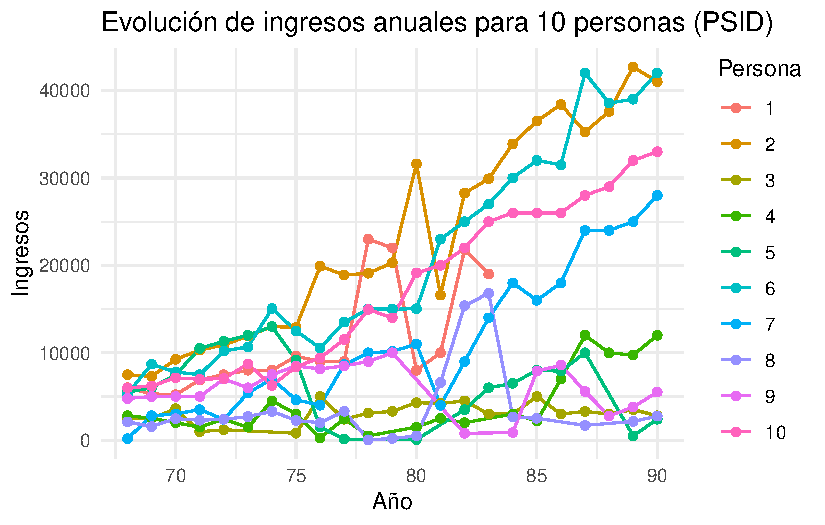
\includegraphics{cap2_files/figure-pdf/unnamed-chunk-1-1.pdf}

Este gráfico muestra la evolución de los ingresos anuales para
diferentes personas a lo largo del tiempo. Se observa que los datos son
heterogéneos y varían significativamente entre individuos, lo que
muestra la dependencia entre observaciones; algo que viola los supuestos
básicos de independencia de las observaciones, fundamentales para
modelos clásicos como la regresión lineal simple.

\begin{verbatim}

Call:
lm(formula = income ~ year, data = psid_subset)

Residuals:
     Min       1Q   Median       3Q      Max 
-17956.7  -7314.1   -380.3   4693.2  24996.3 

Coefficients:
             Estimate Std. Error t value Pr(>|t|)    
(Intercept) -46198.57    7519.91  -6.143 4.02e-09 ***
year           726.46      95.33   7.621 8.65e-13 ***
---
Signif. codes:  0 '***' 0.001 '**' 0.01 '*' 0.05 '.' 0.1 ' ' 1

Residual standard error: 9192 on 209 degrees of freedom
Multiple R-squared:  0.2175,    Adjusted R-squared:  0.2137 
F-statistic: 58.08 on 1 and 209 DF,  p-value: 8.655e-13
\end{verbatim}

En la salida del modelo, vemos cómo el modelo asume que la variabilidad
entre individuos se puede representar con un único coeficiente,
ignorando por completo la dependencia entre observaciones. Además, dicho
coeficiente tiene un valor muy bajo, mostrando que el modelo explica muy
poca variabilidad de los datos y que, por tanto, no nos sirve para
analizar datos longitudinales.

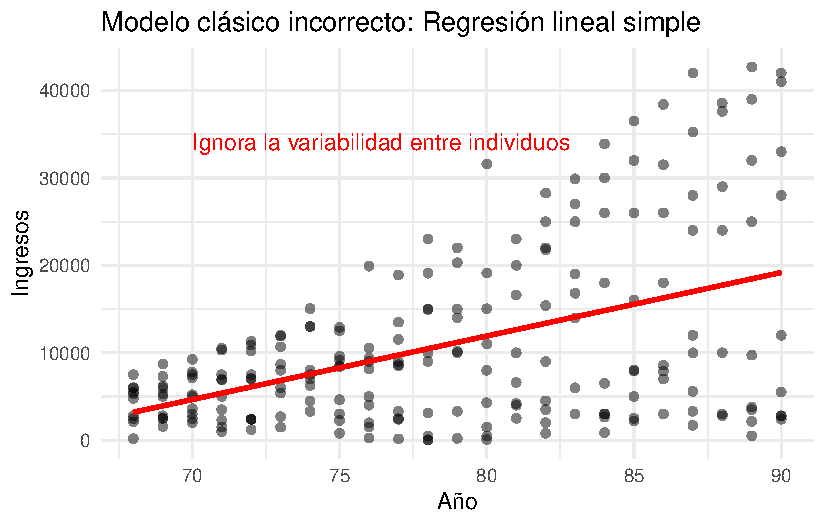
\includegraphics{cap2_files/figure-pdf/unnamed-chunk-3-1.pdf}

Este gráfico muestra cómo la regresión lineal simple aplicada a estos
datos genera una representación distorsionada, ignorando por completo la
correlación de los datos longitudinales; dando lugar a un mal ajuste y a
resultados estadísticos inapropiados que demuestran por qué no debemos
utilizar estadística clásica para este tipo de datos.

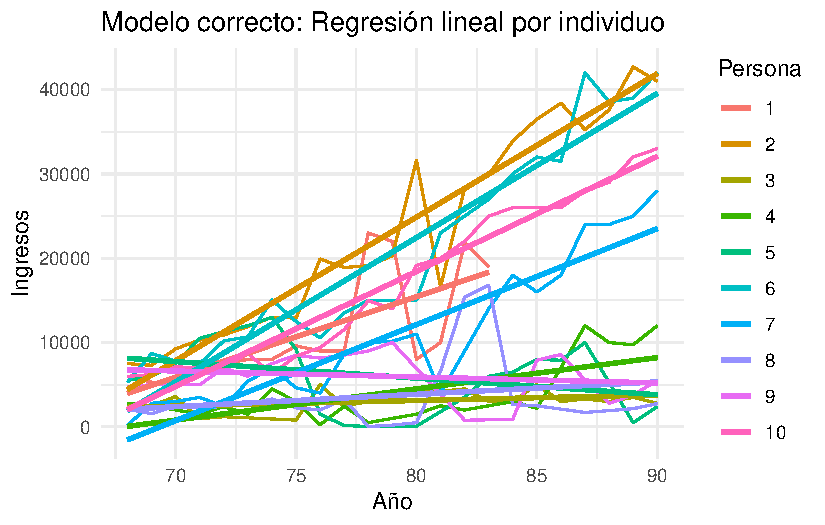
\includegraphics{cap2_files/figure-pdf/unnamed-chunk-4-1.pdf}

En esta gráfica, en la que ajustamos un modelo para cada individuo,
mostrando que las pendientes e interceptos varían significativamente,
destacando la necesidad de modelos mixtos.

\section{Modelos mixtos}\label{modelos-mixtos}

Para analizar datos longitudinales de manera adecuada, se deben emplear
modelos mixtos, que permiten:

\begin{itemize}
\tightlist
\item
  Capturar la variabilidad entre individuos mediante efectos aleatorios.
\item
  Modelar la correlación entre observaciones dentro de una misma unidad.
\item
  Incluir covariables tanto a nivel individual como grupal.
\end{itemize}

\subsection{Ventajas de los modelos
mixtos}\label{ventajas-de-los-modelos-mixtos}

\begin{itemize}
\tightlist
\item
  Flexibilidad para incluir efectos específicos por individuo o grupo.
\item
  Estimación precisa de la incertidumbre, respetando la dependencia
  entre observaciones.
\item
  Generalización a estructuras de datos complejas.
\end{itemize}

\bookmarksetup{startatroot}

\chapter*{Referencias}\label{referencias}
\addcontentsline{toc}{chapter}{Referencias}

\markboth{Referencias}{Referencias}

\phantomsection\label{refs}
\begin{CSLReferences}{0}{1}
\begin{itemize}
\item
  Faraway, J. J. (2006). \emph{Extending the Linear Model with R:
  Generalized Linear, Mixed Effects and Nonparametric Regression
  Models}. Chapman \& Hall/CRC.
\item
  Fernández Hernández, B. (2024). \emph{Modelos mixtos con R}.
\item
  Roback, P., \& Legler, J. (2021). \emph{Beyond Multiple Linear
  Regression: Applied Generalized Linear Models and Multilevel Models in
  R}.
\item
  Subirana, I. (2020). \emph{Análisis de datos longitudinales}.
\end{itemize}

\end{CSLReferences}



\end{document}
